\documentclass[conference]{IEEEtran}
\usepackage[T1]{fontenc}
\usepackage{amsmath,amssymb}
\usepackage{booktabs}
\usepackage{graphicx}
\usepackage{tikz}
\usetikzlibrary{arrows.meta,calc,positioning}
\usepackage[hidelinks]{hyperref}

\newcommand{\code}[1]{\texttt{#1}}

% IEEEtran writes ``Abstract'' followed by an em dash; use a colon instead.
\usepackage{etoolbox}
\makeatletter
\patchcmd{\abstract}{---}{:\ }{}{}
\patchcmd{\abstract}{---}{:\ }{}{}
\patchcmd{\abstract}{---}{:\ }{}{}
\makeatother

\begin{document}

\title{SysMAC: A Verified $3 \times 3$ Output-Stationary\\Systolic Array for Signed 8-bit Matrix Multiplication}

\author{\IEEEauthorblockN{Abhishek Rana, Harshil Valecha, Sushant Yadav, Piyush, and Priyanshu Tomar}}

\maketitle

\begin{abstract}
This paper describes the design, verification and evaluation of SysMAC, a $3 \times 3$ output-stationary systolic array that multiplies signed 8-bit matrices with 32-bit accumulation, written in Verilog-2001. Rows of one matrix and columns of the other enter the array with a one-cycle skew per row and column, so each cell receives matching operand pairs, and a five-state controller sequences loading, a seven-cycle compute phase and result capture. One multiplication takes 10 clock cycles from start to done, and with back-to-back requests the array completes one every 11 cycles. A sequential design with a single multiply-accumulate unit and the same interface needs 29 and 30 cycles respectively, but the array uses nine multipliers to achieve this and only 42.9\% of its cell-cycles do useful work. Correctness is checked against an independent register-level Python model: all nine testbenches pass, and a mutation check that plants twelve realistic design errors one at a time finds every one; it also exposed a gap in the original tests. Open-source synthesis maps the array to 9 DSP blocks. Placed and routed on a Lattice iCE40 HX8K, which has no multiplier blocks, the array reaches 51.2~MHz against 45.6~MHz for the baseline, so it completes a multiplication 3.25 times faster in time, but with 3.6 times the lookup tables; its critical path runs from the controller through the input scheduler into a processing element. We relate the design to current work on fast inner products, machine-discovered matrix multiplication algorithms and structured sparsity, and show which of these ideas pay off at this size.
\end{abstract}

% ======================================================================
\section{Introduction}

The product $C = AB$ of two $N \times N$ matrices is
\begin{equation}
c_{ij} = \sum_{k=0}^{N-1} a_{ik}\, b_{kj},
\label{eq:matmul}
\end{equation}
which requires $N^3$ multiply-accumulate (MAC) operations. A fully connected neural network layer is one such product, and a convolution can be rewritten as one. A general-purpose processor evaluates \eqref{eq:matmul} with three nested loops and a single multiplier, fetching both operands for every MAC.

A systolic array replaces the loops with a grid of identical cells. Operands enter at the edges and move one cell per clock cycle, so each value fetched is reused by every cell it passes. This paper describes the design, verification and evaluation of a small array of this kind. Our contributions are:
\begin{itemize}
\item a modular, synthesisable $3 \times 3$ output-stationary array with a frozen, documented interface;
\item an exact timing analysis, confirmed in simulation and cross-checked against a published closed-form model;
\item a sequential baseline with an identical interface, so both designs run under the same tests;
\item a verification flow built on an independent register-level model, with a reproducible mutation check that measures how well the tests detect real design errors;
\item an analysis of which current research directions in matrix-multiplication hardware help at this scale.
\end{itemize}

Section~\ref{sec:lit} reviews related work, Section~\ref{sec:design} presents the design and the verification method, Section~\ref{sec:results} reports and discusses the results, and Section~\ref{sec:conc} concludes.

% ======================================================================
\section{Literature Review}
\label{sec:lit}

\subsection{Systolic arrays}
Kung and Leiserson introduced systolic arrays as special-purpose VLSI systems built from a few types of simple cells with regular, local connections~\cite{kung1978}. Their matrix multiplier is a hexagonally connected array for band matrices; we cite it for the concept rather than for the rectangular mesh used here. Kung later stated the central argument for the approach~\cite{kung1982}: because each input is used many times inside the array, the computation rate can be high while the input and output bandwidth stays modest.

\subsection{Systolic arrays in machine learning}
The Tensor Processing Unit (TPU) of Jouppi \emph{et al.}~\cite{jouppi2017} brought systolic arrays into production. Its matrix unit contains $256 \times 256$ MACs performing 8-bit multiply-and-adds; activations enter from the left, weights are loaded from the top, and 16-bit products are summed in 32-bit accumulators below the array. Current Google TPUs still use systolic matrix units: $128 \times 128$ up to v5p and $256 \times 256$ in v6e and TPU7x~\cite{tpudocs}. Jacob \emph{et al.}~\cite{jacob2018} show that networks can be trained for integer-only inference with 8-bit operands and 32-bit accumulation, the widths SysMAC uses.

\subsection{Dataflow and utilisation}
Chen, Emer and Sze~\cite{eyeriss2016} classify accelerators by the data that stays fixed inside a processing element: weight stationary, output stationary or no local reuse; Sze \emph{et al.}~\cite{sze2017} survey these choices. Samajdar \emph{et al.} apply the classification to systolic arrays~\cite{scalesim2018} and derive a closed-form runtime for one fold of the array~\cite{scalesim2020}, which we use in Section~\ref{sec:timing}. Their later version~\cite{scalesim3} reports that a $32 \times 32$ array can be $2.86\times$ more energy-efficient than a $128 \times 128$ one because of utilisation. Gemmini~\cite{gemmini2021} supports both output- and weight-stationary dataflows with a clean separation between the processing element and the mesh, which we follow.

\subsection{Current directions in matrix-multiplication hardware}
\emph{Fewer multiplications per inner product.} Winograd's 1968 identity~\cite{winograd1968} computes a pair of products with one multiplication of two sums, plus correction terms that depend on one matrix only. Pogue and Nicolici~\cite{pogue2024} build this into systolic arrays (FIP and FFIP): one processing element with two pre-adders and a $(w{+}1)$-bit multiplier replaces two baseline ones, reaching the same throughput with about half the MAC units at large array sizes, at the cost of a longer critical path that their FFIP variant recovers.

\emph{Machine-discovered algorithms.} AlphaTensor~\cite{alphatensor} found a 47-multiplication scheme for $4 \times 4$ matrices in arithmetic modulo 2, and AlphaEvolve~\cite{alphaevolve} a 48-multiplication scheme for complex $4 \times 4$ matrices. For $3 \times 3$, neither improves Laderman's 23 multiplications~\cite{laderman1976}.

\emph{Sparsity and number formats.} NVIDIA's 2:4 structured sparsity~\cite{mishra2021} and S2TA~\cite{s2ta} skip zero weights with small multiplexers in front of each MAC. The OCP microscaling formats~\cite{ocpmx} share one power-of-two scale across blocks of 32 elements.

\subsection{Position of this work}
These systems are large and target long inner products. A $3 \times 3$ array cannot compete in throughput. Our aim is a small design in which every architectural claim is stated precisely and checked in simulation, and an honest assessment of which of the ideas above apply at this size (Section~\ref{sec:discussion}).

% ======================================================================
\section{Proposed Solution}
\label{sec:design}

\subsection{Specification}
Table~\ref{tab:spec} summarises the design. All module interfaces were fixed in a shared port specification before implementation, so the modules could be developed and tested independently.

\begin{table}[t]
\caption{Design specification}
\label{tab:spec}
\centering
\begin{tabular}{@{}ll@{}}
\toprule
Parameter & Value \\
\midrule
Array size & $3 \times 3$ (array module parameterised in $N$) \\
Operands & signed, 8 bits \\
Accumulators & signed, 32 bits \\
Dataflow & output stationary \\
Input & $A$ and $B$ in parallel, 72 bits each \\
Output & all nine results in parallel, 288 bits \\
Packing & row major, element $(i,k)$ at bits $8(3i+k)$ upward \\
Clock and reset & single clock, synchronous active-high reset \\
\bottomrule
\end{tabular}
\end{table}

\subsection{Architecture}
Fig.~\ref{fig:top} shows the top level. When \code{start} is asserted, the input buffer latches both matrices and the array is cleared. The input scheduler then feeds the array for seven cycles, after which the output registers capture all nine accumulators and hold them while the array is cleared for the next multiplication.

\begin{figure*}[t]
\centering
\resizebox{0.86\textwidth}{!}{% SysMAC top level (systolic_accelerator_top). Solid arrows: data.
% Dashed arrows: control from systolic_controller.
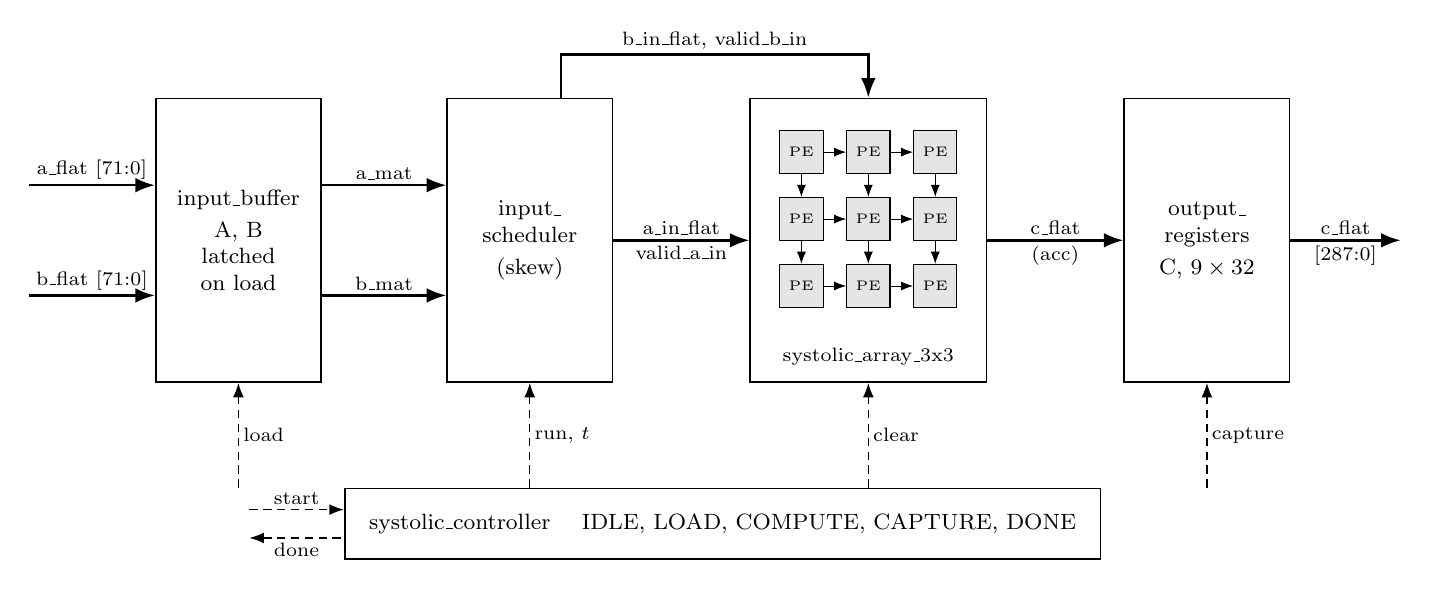
\begin{tikzpicture}[font=\footnotesize, >=Latex,
    blk/.style={draw, line width=0.6pt, minimum height=9mm, minimum width=21mm,
                align=center, fill=white},
    dat/.style={->, line width=0.9pt},
    ctl/.style={->, densely dashed, line width=0.5pt},
    lab/.style={font=\scriptsize, inner sep=1.5pt}]

  \node[blk, minimum height=36mm] (buf) at (0,0) {input\_buffer\\[2pt]A, B\\latched\\on load};
  \node[blk, minimum height=36mm] (sch) at (3.7,0) {input\_\\scheduler\\[2pt](skew)};
  \node[blk, minimum height=36mm, minimum width=30mm] (arr) at (8.0,0) {};
  \node[blk, minimum height=36mm] (out) at (12.3,0) {output\_\\registers\\[2pt]C, $9\times32$};
  \node[blk, minimum width=96mm] (ctrl) at (6.15,-3.6) {systolic\_controller \quad IDLE, LOAD, COMPUTE, CAPTURE, DONE};

  \foreach \i in {0,1,2} {
    \foreach \j in {0,1,2} {
      \node[draw, fill=black!10, minimum size=5.5mm, inner sep=0pt, font=\tiny]
        (pe\i\j) at ($(arr.center)+(-0.85+0.85*\j, 1.12-0.85*\i)$) {PE};
    }
  }
  \foreach \i in {0,1,2} {
    \draw[->, line width=0.3pt] (pe\i0) -- (pe\i1);
    \draw[->, line width=0.3pt] (pe\i1) -- (pe\i2);
    \draw[->, line width=0.3pt] (pe0\i) -- (pe1\i);
    \draw[->, line width=0.3pt] (pe1\i) -- (pe2\i);
  }
  \node[lab, anchor=north] at ($(arr.south)+(0,0.5)$) {systolic\_array\_3x3};

  % host side
  \draw[dat] ($(buf.west)+(-1.6,0.7)$) -- node[lab, above] {a\_flat [71:0]} ($(buf.west)+(0,0.7)$);
  \draw[dat] ($(buf.west)+(-1.6,-0.7)$) -- node[lab, above] {b\_flat [71:0]} ($(buf.west)+(0,-0.7)$);
  \draw[dat] (out.east) -- node[lab, above] {c\_flat} node[lab, below] {[287:0]} ++(1.4,0);

  % data path
  \draw[dat] ($(buf.east)+(0,0.7)$) -- node[lab, above] {a\_mat} ($(sch.west)+(0,0.7)$);
  \draw[dat] ($(buf.east)+(0,-0.7)$) -- node[lab, above] {b\_mat} ($(sch.west)+(0,-0.7)$);
  \draw[dat] (sch.east) -- node[lab, above] {a\_in\_flat} node[lab, below] {valid\_a\_in} (arr.west);
  \draw[dat] ($(sch.north)+(0.4,0)$) -- ++(0,0.55) -| node[lab, above, pos=0.25] {b\_in\_flat, valid\_b\_in} (arr.north);
  \draw[dat] (arr.east) -- node[lab, above] {c\_flat} node[lab, below] {(acc)} (out.west);

  % control
  \draw[ctl] (ctrl.north -| buf.south) -- node[lab, right] {load} (buf.south);
  \draw[ctl] (ctrl.north -| sch.south) -- node[lab, right] {run, $t$} (sch.south);
  \draw[ctl] (ctrl.north -| arr.south) -- node[lab, right] {clear} (arr.south);
  \draw[ctl] (ctrl.north -| out.south) -- node[lab, right] {capture} (out.south);
  \draw[ctl] ($(ctrl.west)+(-1.2,0.18)$) -- node[lab, above] {start} ($(ctrl.west)+(0,0.18)$);
  \draw[ctl, <-] ($(ctrl.west)+(-1.2,-0.18)$) -- node[lab, below] {done} ($(ctrl.west)+(0,-0.18)$);
\end{tikzpicture}
}
\caption{SysMAC top level. Solid arrows carry data; dashed arrows carry control signals from the controller.}
\label{fig:top}
\end{figure*}

\begin{figure*}[t]
\centering
\resizebox{0.9\textwidth}{!}{% Active cells of the 3 x 3 array at each step. PE(i,j) is active for
% i+j <= t <= i+j+2. The same pattern is checked against the RTL after
% every clock edge by tb_systolic_array.v.
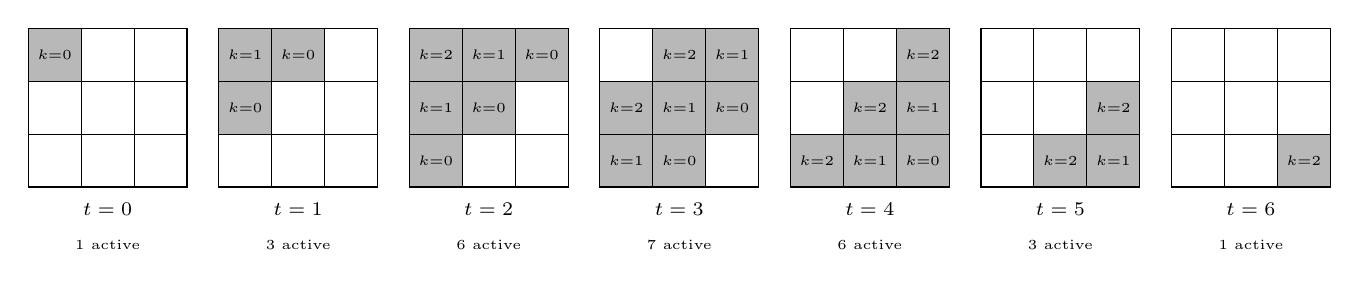
\begin{tikzpicture}[font=\scriptsize, x=0.42cm, y=0.42cm]
  \foreach \t in {0,...,6} {
    \begin{scope}[xshift=\t*2.42cm]
      \foreach \i in {0,1,2} {
        \foreach \j in {0,1,2} {
          \pgfmathtruncatemacro{\lo}{\i+\j}
          \pgfmathtruncatemacro{\hi}{\i+\j+2}
          \pgfmathtruncatemacro{\k}{\t-\i-\j}
          \ifnum\t<\lo
            \draw[line width=0.4pt] (\j*1.6,-\i*1.6) rectangle ++(1.6,-1.6);
          \else\ifnum\t>\hi
            \draw[line width=0.4pt] (\j*1.6,-\i*1.6) rectangle ++(1.6,-1.6);
          \else
            \draw[line width=0.4pt, fill=black!28] (\j*1.6,-\i*1.6) rectangle ++(1.6,-1.6);
            \node[font=\tiny] at (\j*1.6+0.8,-\i*1.6-0.8) {$k{=}\k$};
          \fi\fi
        }
      }
      \pgfmathtruncatemacro{\busy}{(\t<3) ? (\t+1)*(\t+2)/2 : ((\t==3) ? 7 : (7-\t)*(8-\t)/2)}
      \node[anchor=north] at (2.4,-5.0) {$t=\t$};
      \node[anchor=north, font=\tiny] at (2.4,-6.1) {\busy\ active};
    \end{scope}
  }
\end{tikzpicture}
}
\caption{Active cells in each compute cycle, with the index $k$ of the product each cell is computing.}
\label{fig:wave}
\end{figure*}

\subsubsection{Processing element}
Each cell (Fig.~\ref{fig:pe}) registers its two operands and their valid flags and forwards them to its right and lower neighbours. It adds the 16-bit product to its 32-bit accumulator only when both incoming valid flags are set. A \code{clear} signal, asserted while the matrices are loaded, resets every register in the cell.

\begin{figure}[t]
\centering
\resizebox{0.8\columnwidth}{!}{% processing_element: four pass-through registers and one accumulator.
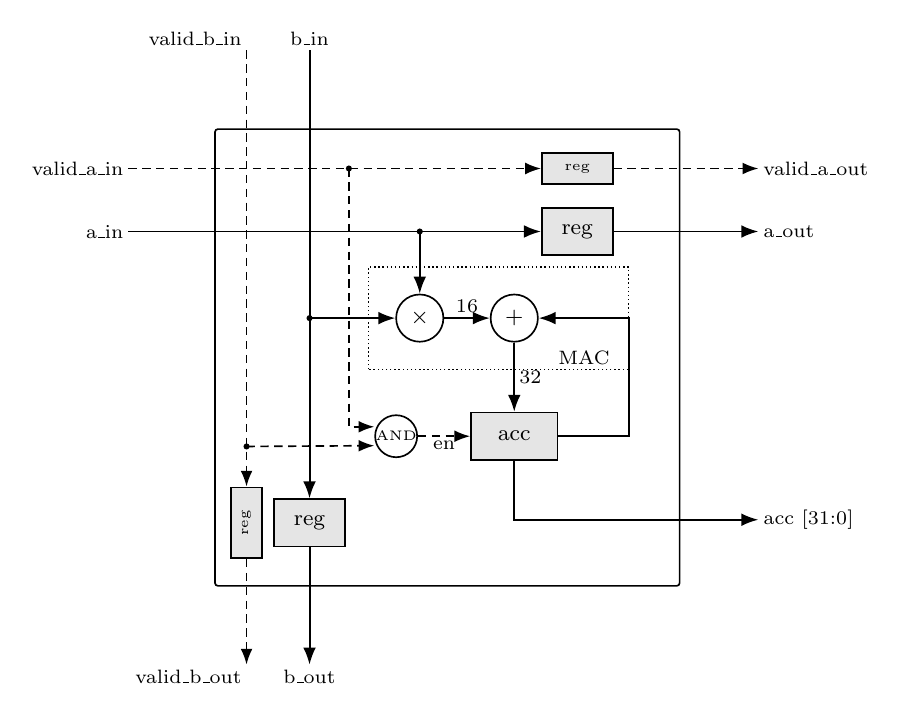
\begin{tikzpicture}[font=\footnotesize, >=Latex,
    reg/.style={draw, line width=0.6pt, minimum width=9mm, minimum height=6mm, fill=black!10},
    sreg/.style={draw, line width=0.6pt, minimum width=9mm, minimum height=4mm, fill=black!10, font=\tiny},
    op/.style={draw, circle, line width=0.6pt, minimum size=6mm, inner sep=0pt},
    w/.style={->, line width=0.7pt},
    v/.style={->, densely dashed, line width=0.6pt},
    lab/.style={font=\scriptsize, inner sep=1.5pt}]

  \draw[line width=0.6pt, rounded corners=1pt] (-2.3,-3.3) rectangle (3.6,2.5);

  % a and valid_a, left to right
  \node[sreg] (rva) at (2.3, 2.0) {reg};
  \node[reg]  (ra)  at (2.3, 1.2) {reg};
  \draw[v] (-3.4,2.0) node[lab, left] {valid\_a\_in} -- (rva.west);
  \draw[v] (rva.east) -- (4.6,2.0) node[lab, right] {valid\_a\_out};
  \draw[w] (-3.4,1.2) node[lab, left] {a\_in} -- (ra.west);
  \draw[w] (ra.east) -- (4.6,1.2) node[lab, right] {a\_out};

  % b and valid_b, top to bottom
  \node[reg]  (rb)  at (-1.1,-2.5) {reg};
  \node[sreg, rotate=90] (rvb) at (-1.9,-2.5) {reg};
  \draw[w] (-1.1,3.5) node[lab, above] {b\_in} -- (rb.north);
  \draw[w] (rb.south) -- (-1.1,-4.3) node[lab, below] {b\_out};
  \draw[v] (-1.9,3.5) node[lab, above left] {valid\_b\_in} -- (rvb.east);
  \draw[v] (rvb.west) -- (-1.9,-4.3) node[lab, below left] {valid\_b\_out};

  % MAC
  \node[op] (mul) at (0.3, 0.1) {$\times$};
  \node[op] (add) at (1.5, 0.1) {$+$};
  \node[reg, minimum width=11mm] (acc) at (1.5,-1.4) {acc};
  \node[op, minimum size=5mm, font=\tiny] (and) at (0.0,-1.4) {AND};
  \draw[w] (0.3,1.2) -- (mul.north);  \fill (0.3,1.2) circle (1.1pt);
  \draw[w] (-1.1,0.1) -- (mul.west);  \fill (-1.1,0.1) circle (1.1pt);
  \draw[w] (mul.east) -- node[lab, above] {16} (add.west);
  \draw[w] (add.south) -- node[lab, right] {32} (acc.north);
  \draw[w] (acc.east) -- ++(0.9,0) |- (add.east);
  \draw[w] (acc.south) -- ++(0,-0.75) -- ++(3.1,0) node[lab, right] {acc [31:0]};

  % accumulate enable
  \draw[v] (-0.6,2.0) |- ($(and.west)+(0,0.12)$);   \fill (-0.6,2.0) circle (1.1pt);
  \draw[v] (-1.9,-1.53) -- ($(and.west)+(0,-0.12)$); \fill (-1.9,-1.53) circle (1.1pt);
  \draw[v] (and.east) -- node[lab, below] {en} (acc.west);

  \draw[densely dotted, line width=0.5pt] (-0.35,-0.55) rectangle (2.95,0.75);
  \node[lab, anchor=south west] at (2.0,-0.55) {MAC};
\end{tikzpicture}
}
\caption{Processing element.}
\label{fig:pe}
\end{figure}

\subsubsection{Input skew}
Cell $(i,j)$ must receive $a_{ik}$ and $b_{kj}$ in the same cycle. A value entering row $i$ takes $j$ cycles to reach column $j$, and a value entering column $j$ takes $i$ cycles to reach row $i$. Delaying row $i$ by $i$ cycles and column $j$ by $j$ cycles aligns the pairs (Fig.~\ref{fig:array}). At compute cycle $t$ the scheduler drives
\begin{equation}
\text{row } i:\; a_{i,\,t-i}, \qquad \text{column } j:\; b_{\,t-j,\,j},
\label{eq:skew}
\end{equation}
when the index lies in $\{0, 1, 2\}$, and zero with the valid flag cleared otherwise. The scheduler is combinational and is the only block that applies skew; the controller supplies an enable and the cycle counter $t$.

\begin{figure}[t]
\centering
\resizebox{0.88\columnwidth}{!}{% 3 x 3 array with the skewed input streams drawn as a staircase.
% The element nearest the array enters first. Empty slots are zeros with
% valid low.
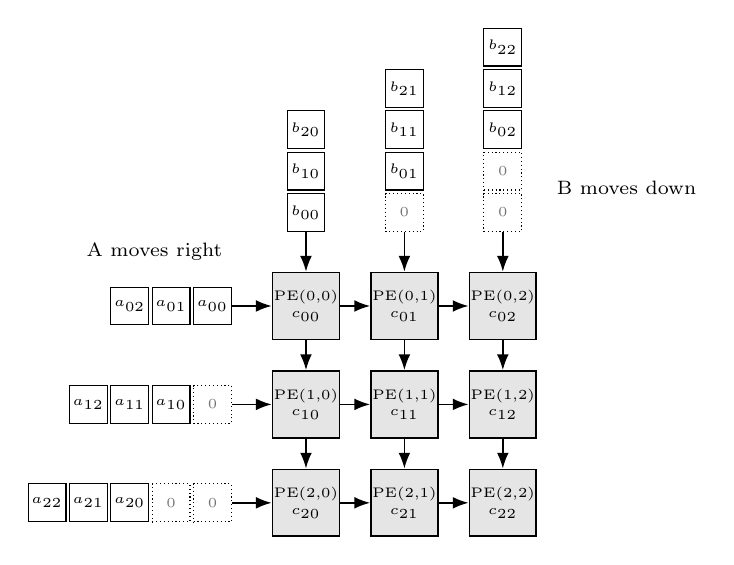
\begin{tikzpicture}[font=\scriptsize, >=Latex, x=1.25cm, y=1.25cm,
    pe/.style={draw, line width=0.6pt, minimum size=8.5mm, fill=black!10, align=center,
               inner sep=0pt, font=\tiny},
    tok/.style={draw, line width=0.4pt, minimum size=4.8mm, inner sep=0pt, font=\tiny},
    gap/.style={draw, densely dotted, line width=0.4pt, minimum size=4.8mm, inner sep=0pt,
                font=\tiny, text=black!55},
    w/.style={->, line width=0.6pt}]

  \foreach \i in {0,1,2} {
    \foreach \j in {0,1,2} {
      \node[pe] (p\i\j) at (\j,-\i) {PE(\i,\j)\\$c_{\i\j}$};
    }
  }
  \foreach \i in {0,1,2} {
    \draw[w] (p\i0) -- (p\i1);
    \draw[w] (p\i1) -- (p\i2);
    \draw[w] (p0\i) -- (p1\i);
    \draw[w] (p1\i) -- (p2\i);
  }

  % A streams on the left: row i has i empty slots before its first element
  \foreach \i in {0,1,2} {
    \foreach \s in {0,1,2,3,4} {
      \pgfmathtruncatemacro{\k}{\s-\i}
      \ifnum\k<0
        \node[gap] (a\i\s) at (-0.95-0.42*\s,-\i) {0};
      \else\ifnum\k<3
        \node[tok] (a\i\s) at (-0.95-0.42*\s,-\i) {$a_{\i\k}$};
      \fi\fi
    }
    \draw[w] (a\i0) -- (p\i0);
  }

  % B streams on the top: column j has j empty slots before its first element
  \foreach \j in {0,1,2} {
    \foreach \s in {0,1,2,3,4} {
      \pgfmathtruncatemacro{\k}{\s-\j}
      \ifnum\k<0
        \node[gap] (b\j\s) at (\j,0.95+0.42*\s) {0};
      \else\ifnum\k<3
        \node[tok] (b\j\s) at (\j,0.95+0.42*\s) {$b_{\k\j}$};
      \fi\fi
    }
    \draw[w] (b\j0) -- (p0\j);
  }

  \node[anchor=east, font=\scriptsize] at (-0.75,0.55) {A moves right};
  \node[anchor=west, font=\scriptsize] at (2.45,1.2) {B moves down};
\end{tikzpicture}
}
\caption{The array and its skewed input streams. The element nearest the array enters first; dotted slots are zeros with the valid flag cleared.}
\label{fig:array}
\end{figure}

\subsubsection{Controller}
The controller is a five-state Moore machine (Fig.~\ref{fig:fsm}). LOAD latches the inputs and clears the array in one cycle, and COMPUTE lasts seven cycles. CAPTURE is needed because the final product is added on the clock edge that ends COMPUTE, so the accumulators are complete only one cycle later. DONE asserts \code{done} for one cycle. A \code{start} outside IDLE is ignored. Fig.~\ref{fig:timing} shows one multiplication.

\begin{figure}[t]
\centering
\resizebox{0.85\columnwidth}{!}{% systolic_controller state machine. Outputs are Moore: each depends only on the state.
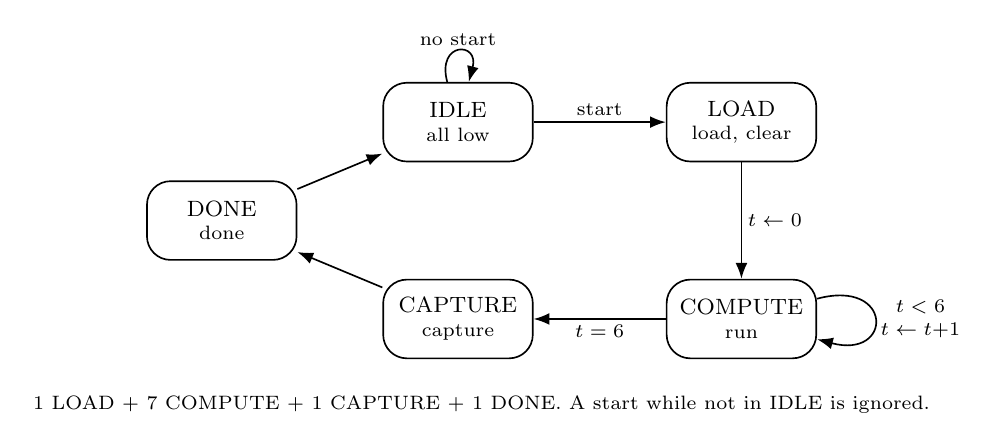
\begin{tikzpicture}[font=\footnotesize, >=Latex,
    st/.style={draw, line width=0.6pt, rounded corners=3mm, minimum width=19mm,
               minimum height=10mm, align=center, fill=white},
    tr/.style={->, line width=0.6pt},
    lab/.style={font=\scriptsize, inner sep=2pt, align=center}]

  \node[st] (idle) at (0,0)      {IDLE\\[-1pt]{\scriptsize all low}};
  \node[st] (load) at (3.6,0)    {LOAD\\[-1pt]{\scriptsize load, clear}};
  \node[st] (comp) at (3.6,-2.5) {COMPUTE\\[-1pt]{\scriptsize run}};
  \node[st] (cap)  at (0,-2.5)   {CAPTURE\\[-1pt]{\scriptsize capture}};
  \node[st] (done) at (-3.0,-1.25) {DONE\\[-1pt]{\scriptsize done}};

  \draw[tr] (idle) -- node[lab, above] {start} (load);
  \draw[tr] (load) -- node[lab, right] {$t \leftarrow 0$} (comp);
  \draw[tr] (comp) -- node[lab, below] {$t = 6$} (cap);
  \draw[tr] (cap)  -- (done);
  \draw[tr] (done) -- (idle);
  \draw[tr] (comp) edge[loop right, looseness=5] node[lab, right] {$t < 6$\\$t \leftarrow t{+}1$} (comp);
  \draw[tr] (idle) edge[loop above, looseness=5] node[lab, above] {no start} (idle);

  \node[lab, anchor=north] at (0.3,-3.4)
    {1 LOAD + 7 COMPUTE + 1 CAPTURE + 1 DONE. A start while not in IDLE is ignored.};
\end{tikzpicture}
}
\caption{Controller state machine and its outputs.}
\label{fig:fsm}
\end{figure}

\begin{figure}[t]
\centering
\resizebox{\columnwidth}{!}{% One job, cycle by cycle. Edge 1 samples start; done is visible after edge 10.
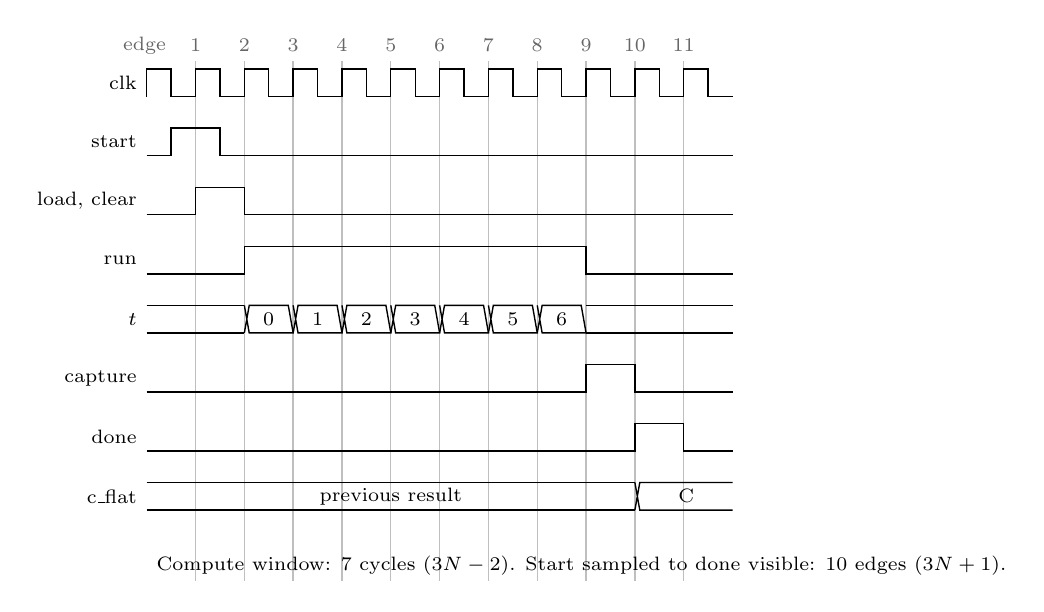
\begin{tikzpicture}[font=\scriptsize, x=0.62cm, y=0.5cm, line width=0.5pt]
  \def\lo{0} \def\hi{0.7}
  % cycle grid: cycle c spans [c, c+1], edge e sits at x = e
  \foreach \e in {1,...,11} {
    \draw[black!25] (\e,0.9) -- (\e,-12.3);
    \node[black!60] at (\e,1.3) {\e};
  }
  \node[anchor=east, black!60] at (0.6,1.3) {edge};

  % helper: a signal high from x1 to x2 on row y
  \newcommand{\sig}[4]{% name, y, x1, x2
    \node[anchor=east] at (0,#2+0.35) {#1};
    \draw (0,#2) -- (#3,#2) -- (#3,#2+\hi) -- (#4,#2+\hi) -- (#4,#2) -- (12,#2);}

  % clock
  \node[anchor=east] at (0,0.35) {clk};
  \foreach \c in {0,...,11} {
    \draw (\c,0) -- (\c,\hi) -- (\c+0.5,\hi) -- (\c+0.5,0) -- (\c+1,0);
  }
  \sig{start}{-1.5}{0.5}{1.5}
  \sig{load, clear}{-3}{1}{2}
  \sig{run}{-4.5}{2}{9}
  % t bus
  \node[anchor=east] at (0,-5.65) {$t$};
  \draw (0,-6) -- (2,-6) (0,-5.3) -- (2,-5.3);
  \foreach \c in {2,...,8} {
    \pgfmathtruncatemacro{\tv}{\c-2}
    \draw (\c,-6) -- (\c+0.1,-5.3) -- (\c+0.9,-5.3) -- (\c+1,-6) -- (\c+0.1,-6) -- (\c,-5.3);
    \node at (\c+0.5,-5.65) {\tv};
  }
  \draw (9,-6) -- (12,-6) (9,-5.3) -- (12,-5.3);
  \sig{capture}{-7.5}{9}{10}
  \sig{done}{-9}{10}{11}
  % c_flat bus
  \node[anchor=east] at (0,-10.15) {c\_flat};
  \draw (0,-10.5) -- (10,-10.5) (0,-9.8) -- (10,-9.8);
  \draw (10,-10.5) -- (10.1,-9.8) -- (12,-9.8) (10,-9.8) -- (10.1,-10.5) -- (12,-10.5);
  \node at (5,-10.15) {previous result};
  \node at (11.05,-10.15) {C};

  \node[anchor=west, align=left] at (0,-11.9)
    {Compute window: 7 cycles ($3N-2$). Start sampled to done visible: 10 edges ($3N+1$).};
\end{tikzpicture}
}
\caption{One multiplication. Edge 1 samples \code{start}; \code{done} and the result are visible after edge 10.}
\label{fig:timing}
\end{figure}

\subsection{Timing analysis}
\label{sec:timing}
From \eqref{eq:skew}, cell $(i,j)$ computes its $k$-th product at
\begin{equation}
t = i + j + k .
\label{eq:when}
\end{equation}
The last product, at cell $(2,2)$ with $k = 2$, occurs at $t = 3(N-1) = 6$, so computing takes $3N - 2 = 7$ cycles and the active cells form a diagonal wavefront (Fig.~\ref{fig:wave}). We count latency from the edge that samples \code{start} to the edge after which \code{done} is visible:
\begin{equation}
L = 1 + 1 + (3N-2) + 1 = 3N + 1 = 10 \text{ cycles}
\label{eq:lat}
\end{equation}
(sample, LOAD, COMPUTE, CAPTURE). SCALE-Sim gives one fold of an array as $2S_R + S_C + T - 2$ cycles~\cite{scalesim2020}, which is $4N - 2 = 10$ for $N = 3$: seven compute cycles plus three to shift results out through the bottom edge. SysMAC reads all accumulators in parallel, so the two agree once the readout method is accounted for.

Only $N^3 = 27$ of the $N^2(3N-2) = 63$ cell-cycles do useful work, a utilisation of 42.9\%, because cells wait for the wavefront and idle after it passes.

\subsection{Accumulator width}
The product of largest magnitude is $(-128)^2 = 16\,384$, so the largest sum of three products is $49\,152$, which needs 17 signed bits; in general $B_{\min} = 2W + \lfloor \log_2 N \rfloor$ for $W$-bit operands, one bit fewer than the commonly quoted $2W + \lceil \log_2 N \rceil$ when $N$ is not a power of two. SysMAC uses 32 bits, following TPU and integer-inference practice~\cite{jouppi2017, jacob2018}.

\subsection{Sequential baseline}
The baseline evaluates \eqref{eq:matmul} with one MAC unit and three counters, one MAC per cycle. It has the same ports and handshake: sample, LOAD and 27 compute cycles give $N^3 + 2 = 29$ cycles in the convention of \eqref{eq:lat}.

\subsection{Verification method}
\label{sec:verif}
\emph{Reference model.} An independent Python model contains three descriptions: the triple loop of \eqref{eq:matmul}, a register-level model of the array advanced one clock edge at a time with both valid flags, and the operation order of the baseline. It checks that they agree with each other and with NumPy on 1560 matrix pairs for $N \in \{2,3,4,5,8\}$, and that every cell is active exactly as \eqref{eq:when} predicts.

\emph{Test data.} The model writes 112 cases (12 directed, 100 random): zeros, the identity on either side, all $-128$, all $127$, $-128$ against $127$, alternating signs, single corner elements, and an asymmetric pair that fails if $B$ is read transposed. For each case it also records the scheduler output and all accumulators after every clock edge.

\emph{Testbenches.} One per level:
\begin{enumerate}
\item \emph{Units:} MAC unit and processing element: signs, valid flags, clear, reset.
\item \emph{Scheduler and array:} scheduler outputs for $t = 0 \ldots 7$ and random matrices; the array against the model after every edge for $N = 3$ (all 112 cases), and final products for $N = 2$ and $4$.
\item \emph{Controller:} state sequence, the seven values of $t$, one-cycle \code{done}.
\item \emph{System:} directed, random and back-to-back jobs, exact latency, reset during a job. A vector testbench drives the 112 model cases into either design, changes the inputs right after LOAD to prove they are latched, and pulses \code{start} during COMPUTE, CAPTURE and DONE, which must all be ignored.
\end{enumerate}

\emph{Mutation check.} A passing test suite is evidence only if it fails on a wrong design. A script copies the repository, plants one realistic error, reruns every testbench, and records which ones fail. One script regenerates the vectors and runs all testbenches with Icarus Verilog 13.

% ======================================================================
\section{Results and Discussion}
\label{sec:results}

\subsection{Functional correctness}
All nine testbench runs pass. The demonstration case $A = [[1,2,3],[4,5,6],[7,8,9]]$, $B = [[9,8,7],[6,5,4],[3,2,1]]$ gives $C = [[30,24,18],[84,69,54],[138,114,90]]$. Table~\ref{tab:trace} shows the accumulators of this job after each clock edge, taken from simulation: $c_{00}$ is complete after edge 5 ($t = 2$), while $c_{22}$ completes only on edge 9, which confirms \eqref{eq:when} and the need for the CAPTURE cycle. Fig.~\ref{fig:wave-sim} shows the same job as recorded by the simulator.

\begin{figure*}[t]
\centering
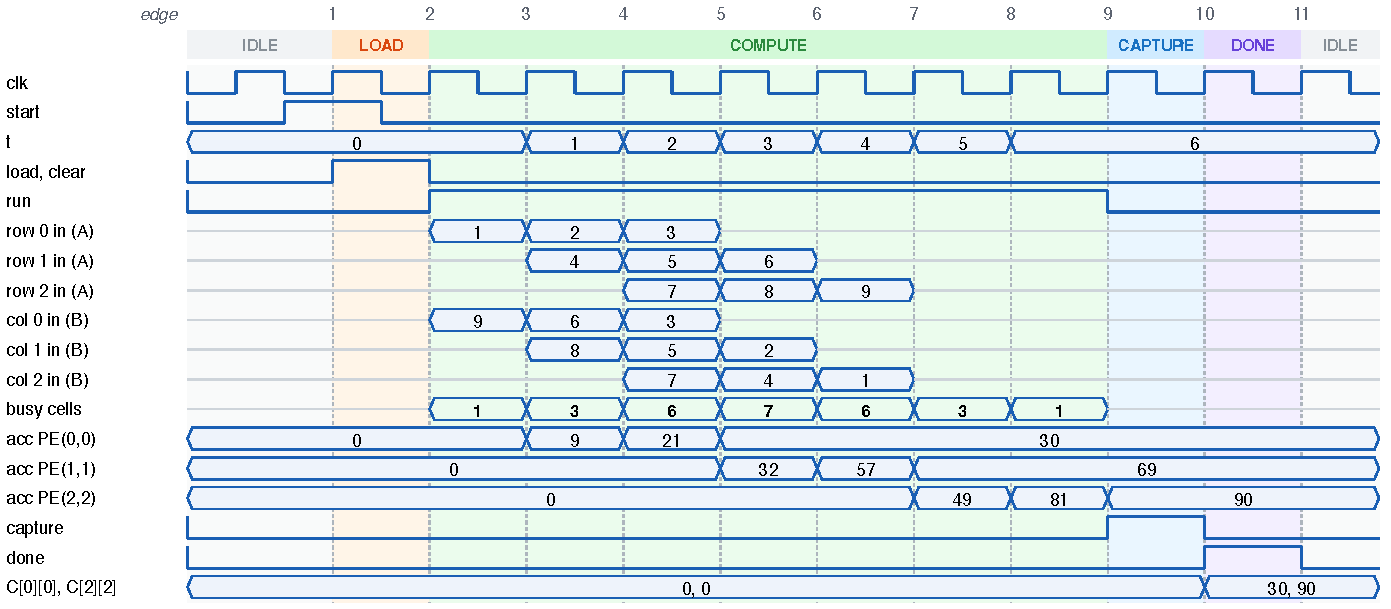
\includegraphics[width=0.72\textwidth]{../docs/figures/waveform.pdf}
\caption{Simulated waveform of the demonstration job, from the testbench's VCD file. Edges are numbered from the one that samples \code{start}; bands are controller states. Operands enter as a staircase, busy cells follow the wavefront $1, 3, 6, 7, 6, 3, 1$, and cell $(2,2)$ finishes on edge 9.}
\label{fig:wave-sim}
\end{figure*}

\begin{table}[t]
\caption{Accumulators after each clock edge, demonstration job (simulation)}
\label{tab:trace}
\centering
\footnotesize
\begin{tabular}{@{}rlcl@{}}
\toprule
Edge & State & $t$ & $c_{00}\, c_{01}\, c_{02}\,/\,c_{10}\, c_{11}\, c_{12}\,/\,c_{20}\, c_{21}\, c_{22}$ \\
\midrule
3 & COMPUTE & 1 & 9 0 0 / 0 0 0 / 0 0 0 \\
4 & COMPUTE & 2 & 21 8 0 / 36 0 0 / 0 0 0 \\
5 & COMPUTE & 3 & 30 18 7 / 66 32 0 / 63 0 0 \\
6 & COMPUTE & 4 & 30 24 15 / 84 57 28 / 111 56 0 \\
7 & COMPUTE & 5 & 30 24 18 / 84 69 48 / 138 96 49 \\
8 & COMPUTE & 6 & 30 24 18 / 84 69 54 / 138 114 81 \\
9 & CAPTURE & 6 & 30 24 18 / 84 69 54 / 138 114 90 \\
10 & DONE & 6 & result on \code{c\_flat}, \code{done} = 1 \\
\bottomrule
\end{tabular}
\end{table}

\subsection{Strength of the tests}
Table~\ref{tab:mut} lists the planted errors. All twelve real errors are detected, most by three or four testbenches. Two findings matter. First, a 16-bit accumulator is not detected by the processing-element testbench, whose sums stay within 16 bits; only the array and system tests catch it. Second, before this check, a controller that restarts when \code{start} arrives during CAPTURE or DONE passed every testbench; the vector testbench was extended to pulse \code{start} in those states. The one surviving change, output registers that copy every cycle, is allowed by the specification, since the result is only guaranteed while \code{done} is high.

\begin{table}[t]
\caption{Planted design errors and the testbenches that detect them}
\label{tab:mut}
\centering
\footnotesize
\begin{tabular}{@{}lp{0.42\columnwidth}@{}}
\toprule
Planted error & Detected by \\
\midrule
$B$ enters one cycle late & scheduler, system, demo, vector \\
$B$ read transposed & scheduler, system, demo, vector \\
unsigned multiplication & PE, array, system, vector \\
accumulator wraps at 16 bits & array, system, vector \\
clear does not reset the PE & PE, array, system, vector \\
clear resets only the accumulator & PE \\
PE ignores \code{valid\_b} & PE, array \\
controller ends one cycle early & controller, system, demo, vector \\
restart on \code{start} in CAPTURE & vector \\
restart on \code{start} in DONE & vector \\
input buffer does not latch & vector \\
baseline does not restart its sum & vector (baseline) \\
output registers copy every cycle & none (allowed by the spec) \\
\bottomrule
\end{tabular}
\end{table}

\subsection{Performance}
Table~\ref{tab:perf} compares the two designs. Latency drops from 29 to 10 cycles ($2.9\times$). With \code{start} held high, the array completes a multiplication every 11 cycles and the baseline every 30, so throughput improves by $2.73\times$. The array pays for this with nine multipliers instead of one: per multiplier it is less busy (42.9\% against 100\%). Its real advantage is scaling: latency grows as $3N + 1$ for the array and $N^3 + 2$ for the baseline, so the cycle ratio is $5.1\times$ at $N = 4$ and $20.6\times$ at $N = 8$ (derived).

\begin{table}[t]
\caption{Systolic array and sequential baseline}
\label{tab:perf}
\centering
\begin{tabular}{@{}lrr@{}}
\toprule
 & Systolic & Baseline \\
\midrule
Multipliers & 9 & 1 \\
Latency, start to done (cycles) & 10 & 29 \\
Throughput, cycles per job & 11 & 30 \\
Multiplier utilisation & 42.9\% & 100\% \\
DSP48E1 (Yosys) & 9 & 1 \\
Flip-flops, hierarchical / flattened & 602 / 446 & 474 / 474 \\
LUTs, hierarchical / flattened & 144 / 118 & 408 / 408 \\
\bottomrule
\end{tabular}
\end{table}

\subsection{Resources and timing}
Yosys 0.71 \code{synth\_xilinx} reports no latches or structural problems. The flip-flop count depends on the flow: with module boundaries kept, every processing element keeps its forwarding registers, including those at the right and bottom edges that nothing reads (602); flattening removes them (446). The baseline needs more lookup tables than the array, because it selects one of nine operands every cycle. A longest-path analysis of the flattened netlist gives 85 gate levels from the controller's counter $t$, through the scheduler's index arithmetic and operand selection, into the multiply-add of an edge cell. The clock is therefore likely limited by the scheduler and the MAC together rather than by the MAC alone; registering the scheduler outputs would shorten this path for one cycle of latency. Artix-7 clock frequency and power require Vivado; an out-of-context script is included in the repository, because the top's 436 port bits exceed the user I/O of small Artix-7 packages.

\emph{Place and route.} To measure the clock frequency with open-source tools, both designs were also synthesised for a Lattice iCE40 HX8K (CT256 package) and placed and routed with nextpnr-ice40 0.11.1 under a 50~MHz constraint. Because the maximum frequency $f_{\max}$ depends on the placer's random seed, we report the median over seeds 1 to 5 (range 46.8 to 52.3~MHz for the array, 45.3 to 46.3~MHz for the baseline). The iCE40 has fewer pins than the design has port bits and nextpnr has no out-of-context mode, so for place and route each design sits in a harness that fills $A$ and $B$ from a shift register and shifts $C$ out; every port is registered, so the timed paths lie inside the design. Resource counts are for the bare design. Table~\ref{tab:ice40} lists the results.

\begin{table}[t]
\caption{Placed and routed on an iCE40 HX8K (50~MHz constraint)}
\label{tab:ice40}
\centering
\begin{tabular}{@{}lrr@{}}
\toprule
 & Systolic & Baseline \\
\midrule
4-input LUTs (of 7680) & 3256 & 909 \\
Flip-flops & 830 & 474 \\
$f_{\max}$, median of 5 seeds (MHz) & 51.2 & 45.6 \\
Latency, start to done (ns) & 195.4 & 635.8 \\
Throughput, ns per job & 214.9 & 657.8 \\
LUTs $\times$ latency (LUT$\cdot\mu$s) & 636 & 578 \\
\bottomrule
\end{tabular}
\end{table}

The critical path of the array runs from the controller's counter $t$ through the scheduler and the multiply-add into a cell accumulator (19.5~ns for seed~1, 57\% of it routing), which confirms the gate-level analysis above. The baseline's path, through its nine-way operand selection and the multiply-add, is slightly longer (21.9~ns), so the array does not pay for its parallelism with a slower clock. It is therefore 3.25 times faster in latency and 3.06 times faster in throughput, slightly more than the cycle ratios. Without multiplier blocks, however, it needs 3.6 times the lookup tables, and its product of lookup tables and latency is about 10\% higher than the baseline's: at this size the speed-up is bought with a proportional amount of logic, which follows from its 42.9\% utilisation.

\subsection{Discussion: what current research offers at this size}
\label{sec:discussion}
\emph{Utilisation.} Overlapping consecutive jobs hides fill and drain. If job $n$'s product $k$ reaches cell $(i,j)$ at $t = i + j + 3n + k$, $J$ jobs take $3J + 4$ compute cycles and utilisation becomes $3J/(3J+4)$: 75\% for $J = 4$ and 92.3\% for $J = 16$ (derived). This is the most direct improvement for SysMAC and needs a first/last tag that travels with the data.

\emph{Fast inner products.} Applying Winograd's identity~\cite{winograd1968, pogue2024} with the inner dimension padded to four needs $9 \times 2$ pair products plus three row and three column corrections: 24 multiplications instead of 27, or 21 if the column terms are precomputed for fixed weights, and six compute cycles instead of seven (derived). The multipliers widen to $9 \times 9$, and the correction overhead grows with $N$ while the array grows with $N^2$, so the saving is small at $3 \times 3$ and grows for larger arrays, consistent with the large-array results in~\cite{pogue2024}.

\emph{Machine-discovered algorithms.} The best known $3 \times 3$ scheme still uses 23 multiplications~\cite{laderman1976, alphaevolve}. Its operands are sums of up to seven matrix entries, which widens multipliers to about 11 bits and needs data from non-neighbouring cells; by a $w^2$ area estimate, 23 such multipliers cost more than 27 plain $8 \times 8$ ones (derived). These algorithms do not pay off in a small systolic array.

\emph{Sparsity and formats.} With an inner dimension of three there is a single padded group of four, so 2:4 sparsity~\cite{mishra2021, s2ta} saves at most one cycle. MXINT8~\cite{ocpmx} would leave the integer array unchanged and add a shared exponent per output.

\subsection{Limitations}
Clock frequency is measured only on the iCE40, a slow device without multiplier blocks, and inside a harness; Artix-7 timing, power and on-board operation are not measured. The array is fixed at $3 \times 3$ at the top level, the parallel 436-bit interface is not realistic for a pin-limited FPGA, and the baseline is a simple counter-based datapath rather than a processor.

% ======================================================================
\section{Individual Contributions}
\label{sec:contrib}
\begin{center}
\begin{tabular}{@{}lp{0.68\columnwidth}@{}}
\toprule
Member & Contribution \\
\midrule
Abhishek Rana & MAC unit and processing element, with their testbenches \\
Harshil Valecha & Port specification, controller, top-level integration, controller, system and demonstration testbenches, repository and code review, prototype video, iCE40 place and route and timing analysis, waveform figure, demonstration script \\
Sushant Yadav & Parameterised $N \times N$ array with $3 \times 3$ wrapper, and its testbench for $N = 2, 3, 4$ \\
Piyush & Input buffer, input scheduler, output registers, scheduler testbench \\
Priyanshu Tomar & Reference model and test data, simulation script, sequential baseline and vector testbench, mutation check, synthesis scripts, block diagrams, README, reports \\
\bottomrule
\end{tabular}
\end{center}

% ======================================================================
\section{Conclusion}
\label{sec:conc}
SysMAC multiplies signed 8-bit $3 \times 3$ matrices in 10 cycles of latency and 11 cycles per job, against 29 and 30 for a one-multiplier baseline with the same interface. Every timing claim follows from the skew rule $t = i + j + k$, is confirmed cycle by cycle in simulation, and agrees with a published runtime model. Verification against an independent model, together with a mutation check that detects all twelve planted errors, gives strong evidence of correctness, and the mutation check itself found and closed a gap in the original tests. The array's cost is visible in the results: nine multipliers, 42.9\% utilisation for an isolated job, and a likely critical path through the input scheduler. Placed and routed on an iCE40, the array also runs at a slightly higher clock than the baseline and is 3.25 times faster in time, at 3.6 times the logic. Overlapping jobs, registering the scheduler outputs and a fast inner-product cell are the natural next steps, and Vivado implementation on the Artix-7, where the multipliers map to DSP blocks, would complete the time and area comparison.

\begin{thebibliography}{00}
\bibitem{kung1978} H. T. Kung and C. E. Leiserson, ``Systolic arrays (for VLSI),'' in \emph{Sparse Matrix Proceedings 1978}, I. S. Duff and G. W. Stewart, Eds. Philadelphia, PA, USA: SIAM, 1979, pp. 256-282.
\bibitem{kung1982} H. T. Kung, ``Why systolic architectures?,'' \emph{Computer}, vol. 15, no. 1, pp. 37-46, Jan. 1982, doi: 10.1109/MC.1982.1653825.
\bibitem{jouppi2017} N. P. Jouppi \emph{et al.}, ``In-datacenter performance analysis of a tensor processing unit,'' in \emph{Proc. 44th Annu. Int. Symp. Comput. Archit. (ISCA)}, 2017, pp. 1-12, doi: 10.1145/3079856.3080246.
\bibitem{tpudocs} Google Cloud, ``TPU system architecture,'' Cloud TPU documentation, 2025. [Online]. Available: https://cloud.google.com/tpu/docs/system-architecture-tpu-vm
\bibitem{jacob2018} B. Jacob \emph{et al.}, ``Quantization and training of neural networks for efficient integer-arithmetic-only inference,'' in \emph{Proc. IEEE/CVF Conf. Comput. Vis. Pattern Recognit. (CVPR)}, 2018, pp. 2704-2713, doi: 10.1109/CVPR.2018.00286.
\bibitem{eyeriss2016} Y.-H. Chen, J. Emer, and V. Sze, ``Eyeriss: A spatial architecture for energy-efficient dataflow for convolutional neural networks,'' in \emph{Proc. 43rd Annu. Int. Symp. Comput. Archit. (ISCA)}, 2016, pp. 367-379, doi: 10.1109/ISCA.2016.40.
\bibitem{sze2017} V. Sze, Y.-H. Chen, T.-J. Yang, and J. S. Emer, ``Efficient processing of deep neural networks: A tutorial and survey,'' \emph{Proc. IEEE}, vol. 105, no. 12, pp. 2295-2329, Dec. 2017, doi: 10.1109/JPROC.2017.2761740.
\bibitem{scalesim2018} A. Samajdar, Y. Zhu, P. Whatmough, M. Mattina, and T. Krishna, ``SCALE-Sim: Systolic CNN accelerator simulator,'' arXiv:1811.02883, 2018.
\bibitem{scalesim2020} A. Samajdar, J. M. Joseph, Y. Zhu, P. Whatmough, M. Mattina, and T. Krishna, ``A systematic methodology for characterizing scalability of DNN accelerators using SCALE-Sim,'' in \emph{Proc. IEEE Int. Symp. Perform. Anal. Syst. Softw. (ISPASS)}, 2020, pp. 58-68.
\bibitem{scalesim3} R. Raj \emph{et al.}, ``SCALE-Sim v3: A modular cycle-accurate systolic accelerator simulator for end-to-end system analysis,'' arXiv:2504.15377, 2025.
\bibitem{gemmini2021} H. Genc \emph{et al.}, ``Gemmini: Enabling systematic deep-learning architecture evaluation via full-stack integration,'' in \emph{Proc. 58th ACM/IEEE Design Autom. Conf. (DAC)}, 2021, pp. 769-774, doi: 10.1109/DAC18074.2021.9586216.
\bibitem{winograd1968} S. Winograd, ``A new algorithm for inner product,'' \emph{IEEE Trans. Comput.}, vol. C-17, no. 7, pp. 693-694, Jul. 1968, doi: 10.1109/TC.1968.227420.
\bibitem{pogue2024} T. E. Pogue and N. Nicolici, ``Fast inner-product algorithms and architectures for deep neural network accelerators,'' \emph{IEEE Trans. Comput.}, vol. 73, no. 2, pp. 495-509, Feb. 2024, doi: 10.1109/TC.2023.3334140.
\bibitem{alphatensor} A. Fawzi \emph{et al.}, ``Discovering faster matrix multiplication algorithms with reinforcement learning,'' \emph{Nature}, vol. 610, pp. 47-53, 2022, doi: 10.1038/s41586-022-05172-4.
\bibitem{alphaevolve} A. Novikov \emph{et al.}, ``AlphaEvolve: A coding agent for scientific and algorithmic discovery,'' arXiv:2506.13131, 2025.
\bibitem{laderman1976} J. D. Laderman, ``A noncommutative algorithm for multiplying $3 \times 3$ matrices using 23 multiplications,'' \emph{Bull. Amer. Math. Soc.}, vol. 82, no. 1, pp. 126-128, 1976, doi: 10.1090/S0002-9904-1976-13988-2.
\bibitem{mishra2021} A. Mishra \emph{et al.}, ``Accelerating sparse deep neural networks,'' arXiv:2104.08378, 2021.
\bibitem{s2ta} Z.-G. Liu, P. N. Whatmough, Y. Zhu, and M. Mattina, ``S2TA: Exploiting structured sparsity for energy-efficient mobile CNN acceleration,'' in \emph{Proc. IEEE Int. Symp. High-Perform. Comput. Archit. (HPCA)}, 2022, arXiv:2107.07983.
\bibitem{ocpmx} Open Compute Project, ``OCP Microscaling Formats (MX) Specification,'' version 1.0, Sep. 2023.
\end{thebibliography}

\end{document}
